% Metódy inžinierskej práce

\documentclass[10pt,twoside,slovak,a4paper]{article}

\usepackage[slovak]{babel}
%\usepackage[T1]{fontenc}
\usepackage[IL2]{fontenc} % lepšia sadzba písmena Ľ než v T1
\usepackage[utf8]{inputenc}
\usepackage{graphicx}
\usepackage{url} % príkaz \url na formátovanie URL
\usepackage{hyperref} % odkazy v texte budú aktívne (pri niektorých triedach dokumentov spôsobuje posun textu)

\usepackage{cite}
%\usepackage{times}

\pagestyle{headings}

\title{Moodle ako nástoj na výučbu matematiky a jeho použitie v e-learnigu\thanks{Semestrálny projekt v predmete Metódy inžinierskej práce, ak. rok 2020/21, vedenie: Jozef Sitarčík}} % meno a priezvisko vyučujúceho na cvičeniach

\author{Samuel Krempaský\\[2pt]
	{\small Slovenská technická univerzita v Bratislave}\\
	{\small Fakulta informatiky a informačných technológií}\\
	{\small \texttt{xkrempasky@stuba.sk}}
	}

\date{\small 8. november 2020} % upravte



\begin{document}

\maketitle

\begin{abstract}
Prostredia e-learningu môžu prispieť k procesu výučby a učenia, pokiaľ sú správne integrované. Tvorba vlastných riešení však vyžaduje programovacie schopnosti a čas. Alternatívou môže byť 
použitie už vytvoreného CMS (Course Management Sytem). Moodle (Modular Object-Oriented Dynamic Learning Environment) si postupne získava popularitu vo svete, ako systém riadenia kurzov pre e-learning. Napriek tomu že je dostupných viacero podobných riešení, aj medzi nimi sa dajú nájsť rozdiely. Tento článok sa venuje porovnaniu s inými technológiami, sumarizáciou ich využiteľnosti a vlastností pre pre použitie v procese e-learningu. Napriek tomu že je dostupných veľa podobných riešení, aj medzi nimi sa dajú nájsť rozdiely.
\end{abstract}



\section{Úvod}

Moodle je open-source čo umožňuje prispôsobiť systém individuálnym potrebám a požiadavkám. Je prostredím, ktoré umožní vzájomnú spoluprácu študentov či už samostatne alebo popri tradičnej výučbe v triede.

Článok v časti~\ref{porovnanie} uvádza prehľad nástrojov podobných technológii Moodle. Ďalej v časti~\ref{moodle} sa zameriava na samotný nástroj Moodle. V časti \ref{použiteľnosť} sa však zameria na porovnanie tejto technológie s ostatnými ktoré boli spomenuté v čast~\ref{porovnanie}. Časti~\ref{funkcie} a~\ref{rozsirenia} bližšie popisujú funkcie nástroja Moodle a možnosti ich prípadného rozšírenia. Záverečné poznámky spolu s krátkym zhrnutím prináša časť~\ref{zaver}.



\section{Prehľad nástrojov pre použitie v e-learningu, alternatívy pre Moodle a ich rozdiely} \label{porovnanie}
Okrem platformy Moodle je možné nájsť množstvo nástrojov s podobným alebo alternatívnym prístupom a možnosťami ako využíva Moodle. Vybrané preto sú majoritné alternatívy - Blackboard, Google Classroom, Chamilo. Porovnanie záujmov o tieto výrazy v Google Trends pre obdobie 11/2019 až 11/2020 jasne ukazuje ich popularitu vo svete na obr.~\ref{f:stats}. Dôležité je aj merítko geografickej polohy, nakoľko napríklad na území Slovenska sa teší obľube Moodle, viď. obr.~\ref{f:statsSK}. 

\begin{figure*}[tbh]
\centering
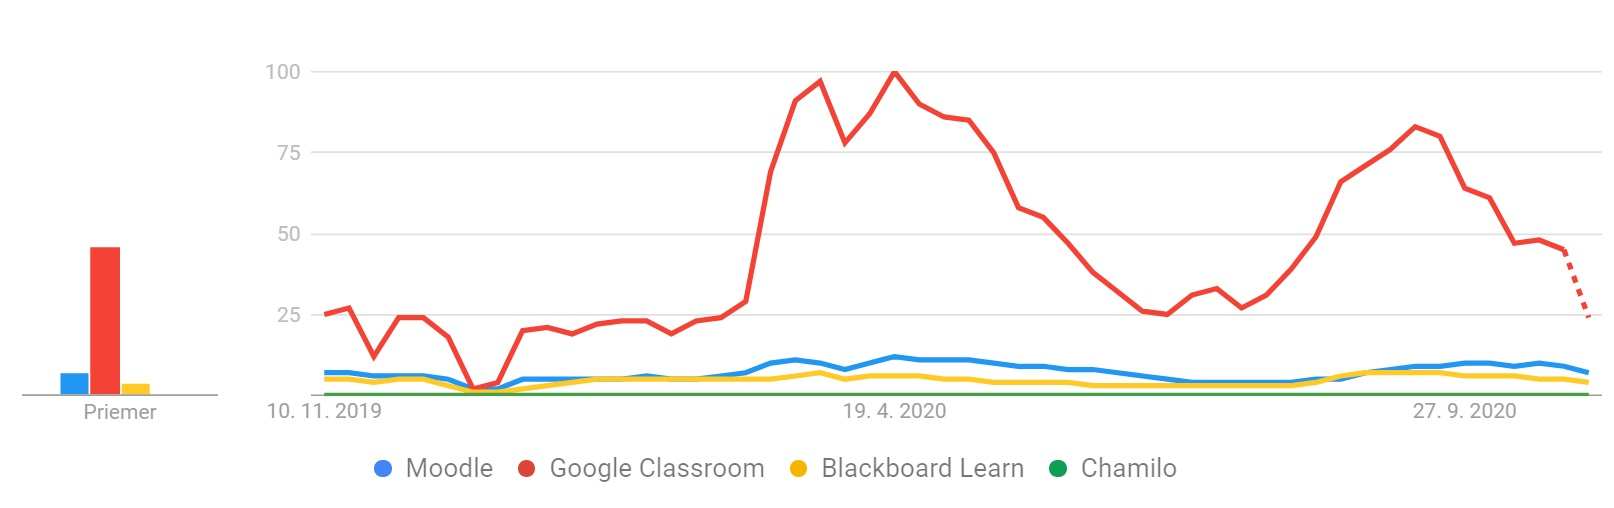
\includegraphics[width=\textwidth]{diagram.jpg}
%Aj text môže byť prezentovaný ako obrázok. Stane sa z neho označný plávajúci objekt. Po vytvorení diagramu zrušte znak \texttt{\%} pred príkazom \verb|\includegraphics| označte tento riadok ako komentár (tiež pomocou znaku \texttt{\%}).
\caption{Porovnanie podľa Google Trends - územie celý svet}
\label{f:stats}
\end{figure*}

\begin{figure*}[tbh]
\centering
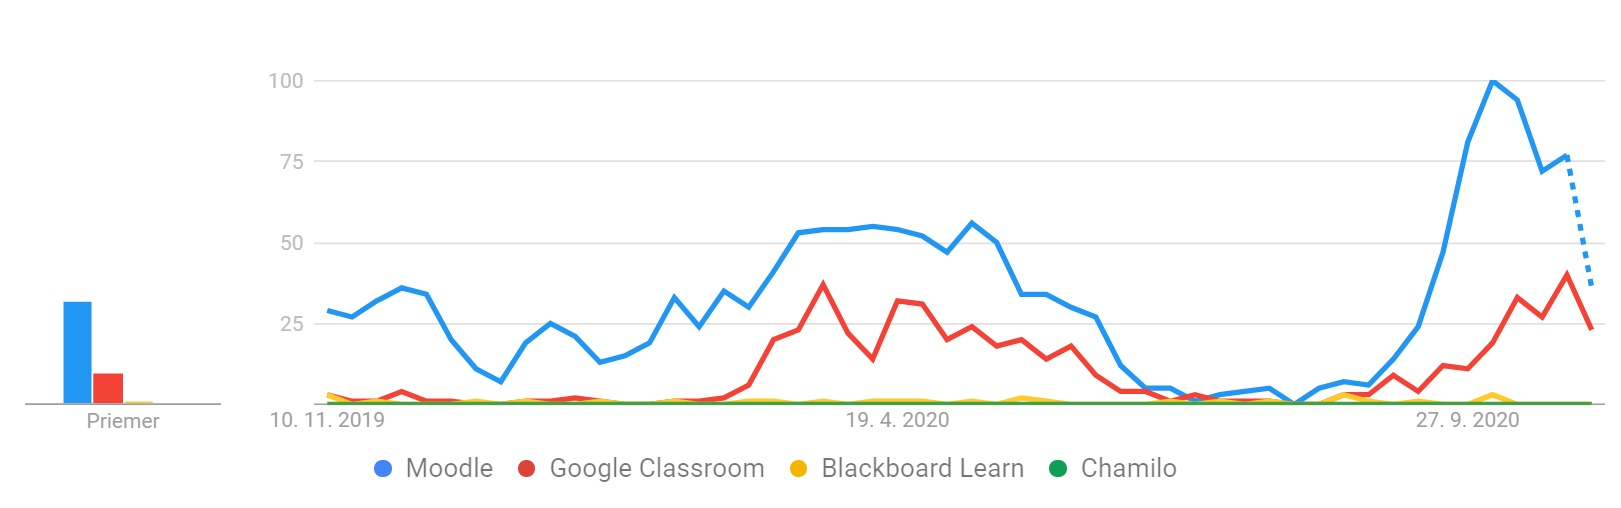
\includegraphics[width=\textwidth]{diagramSK.jpg}
%Aj text môže byť prezentovaný ako obrázok. Stane sa z neho označný plávajúci objekt. Po vytvorení diagramu zrušte znak \texttt{\%} pred príkazom \verb|\includegraphics| označte tento riadok ako komentár (tiež pomocou znaku \texttt{\%}).
\caption{Porovnanie podľa Google Trends - územie Slovensko}
\label{f:statsSK}
\end{figure*}



\section{Moodle ako nástroj v e-learningu } \label{moodle}
Moodle ako nástroj v e-learningu je možné použiť viacerými spôsobmi. Podľa TAM \footnote{ ,,Technology acceptance model'' - \url{https://en.wikipedia.org/wiki/Technology_acceptance_model}} je dôležitý postoj k danej technológii a rozdeľuje ho do 3 kategórií. Tento model pozoruje na používaní nástroja Moodle aj štúdia \cite{hsu2013extended}. 

Pre e-learnig ponúka Moodle viacero vhodných funkcií. Jeden z konceptov je využívanie tohoto nástroja ako banky informácií či akéhosi správcu informácií. Takto bolo Moodle najčastejšie používaný medzi vysokoškolskými študentmi aj v štúdii, kde bola potvrdená hypotéza, že Moodle sa používa hlavne ako úložisko materiálov a informácií \cite{costa2012use}.  


\section{Použiteľnosť nástroja Moodle v porovnaní s alternatívami } \label{pouzitelnost}

\subsection{Blackoboard} \label{pouzitelnost:blackboard}

Blackoboard sa javí ako vhodná alternatíve pre Moodle, avšak v prieskume medzi študentami uspel viac Moodle. 75\% študentov uviedlo že jednoduchší na používanie sa im zdá Moodle \cite{machado2007blackboard}.

\subsection{Google Classroom} \label{pouzitelnost:classroom}

Google Classroom sa javí viac ako rovnocenná alternatíva, množstvom a použiteľnosťou si je rovný s platformou Moodle \cite{barmanfacilitating} . 


\section{Prehľad možností a funkcií nástroja Moodle} \label{funkcie}

E-learningové prostrediach založené na obsahu učiva sú potrebné. Učitelia nemajú čas na ich vlastnú výstavbu. Je preto dôležité vytvoriť prostredie podľa potrieb učiteľa, podľa obsahu či typu učiva. Nakoľko dizajn Moodle je založený na sociálno-konštruktivistickej pedagogike \cite{klaus2005you}, umožňuje ľahké a príjemné používanie prostredia čo vedie k porozumeniu a rozvoju záujmu aj o predmety, ktoré sa považujú za ťažko naučiteľné, za ktoré sú považované predmety ako matematika.


\section{Rozšírenia Moodle a ich využitie v praxi} \label{rozsirenia}
Kedže je Moodle open-source projekt, celý jeho zdrojový kód je voľný dostupný a je preto vhodný pre akékoľvek rozširovanie, či upravovanie. Ku dňu publikovania článku sa nachádza na stránkach Moodle.com 1745 pluginov, z toho 146 tém upravujúcich vzhľad, ktorými je možné si základné funkcie obohatiť, alebo vylepšiť \cite{Moodle:plugins}.

Témy sú rozšírenia ktoré umožňujú alebo priamo menia vzhľad a rozloženie prvkov prostredia. 

Pluginy sú rozšírenia ktoré pridávajú funkcionality alebo upravujú funkcie už samotného jadra. 



\section{Záver} \label{zaver}




%\acknowledgement{Ak niekomu chcete poďakovať\ldots}



\bibliography{literatura}
\bibliographystyle{plain}
\end{document}
